\chapter{Theoretical Background}
\label{ch:theory}

This chapter introduces all mathematical concepts required to derive and
understand the Cartesian impedance controller used in this thesis.
The presentation follows a deliberate step-by-step order:
it begins with the geometry of coordinate frames, builds up the algebraic
tools for transformations, defines the controlled variable as the
end-effector position and orientation, derives the error signal, and then
develops the kinematic and dynamic machinery that connects joint torques
to Cartesian forces.
%% ─────────────────────────────────────────────────────────────
\section{Coordinate Systems}
\label{sec:coord_systems}
%% ─────────────────────────────────────────────────────────────

To describe the motion of a robotic manipulator, multiple coordinate
frames are used simultaneously \cite{Siciliano2009, Craig2005}.
A \textbf{coordinate frame} is a right-handed orthogonal system of
three mutually perpendicular unit vectors anchored at a chosen origin.
For the joint frames, this thesis follows the
\textbf{Denavit--Hartenberg} (\abbr{DH}) convention, a standard robotics
method for assigning coordinate frames to consecutive links in a kinematic
chain \cite{Denavit1955, Craig2005}.
Three frames are central to this work:

\begin{itemize}
  \item \textbf{Base frame} $\{0\}$: fixed to the robot mounting
        surface. Its origin is the robot base reference point used by
        the kinematic model. For the upright Panda configuration used in
        this thesis, the $z_0$-axis points normal to the mounting surface
        and is aligned with the first joint axis, while the $x_0$- and
        $y_0$-axes lie in the mounting plane and complete a right-handed
        coordinate system according to the manufacturer convention.
        All positions, orientations, and forces are ultimately expressed in
        this frame unless stated otherwise.
  \item \textbf{Joint frames} $\{1\},\{2\},\ldots,\{n\}$: rigidly
        attached to the successive links of the kinematic chain.
        The origin of frame $\{i\}$ is placed at the reference point of
        joint $i$ used by the Denavit--Hartenberg model. Its $z_i$-axis
        is the rotation axis of joint $i$; its $x_i$-axis is chosen along
        the common normal to the neighbouring joint axes, and $y_i$
        completes the right-handed frame. These frames move with the
        robot and encode the relative geometry between consecutive links.
  \item \textbf{End-effector frame} $\{EE\}$: attached to the tool
        centre point. Its origin is the controlled point at the tool tip
        or flange, depending on the selected tool definition. The axes
        describe the tool orientation: $z_{EE}$ is taken as the tool approach
        direction, while $x_{EE}$ and $y_{EE}$ span the tool plane and complete
        a right-handed frame. The position and orientation of $\{EE\}$
        relative to $\{0\}$ constitute the controlled position and orientation of the robot.
\end{itemize}

The coordinate-frame assignment and the corresponding Denavit--Hartenberg convention for assigning consecutive coordinate systems
are illustrated in \cref{fig:coordinate_frame_robot}.
\begin{figure}[H]
    \centering
    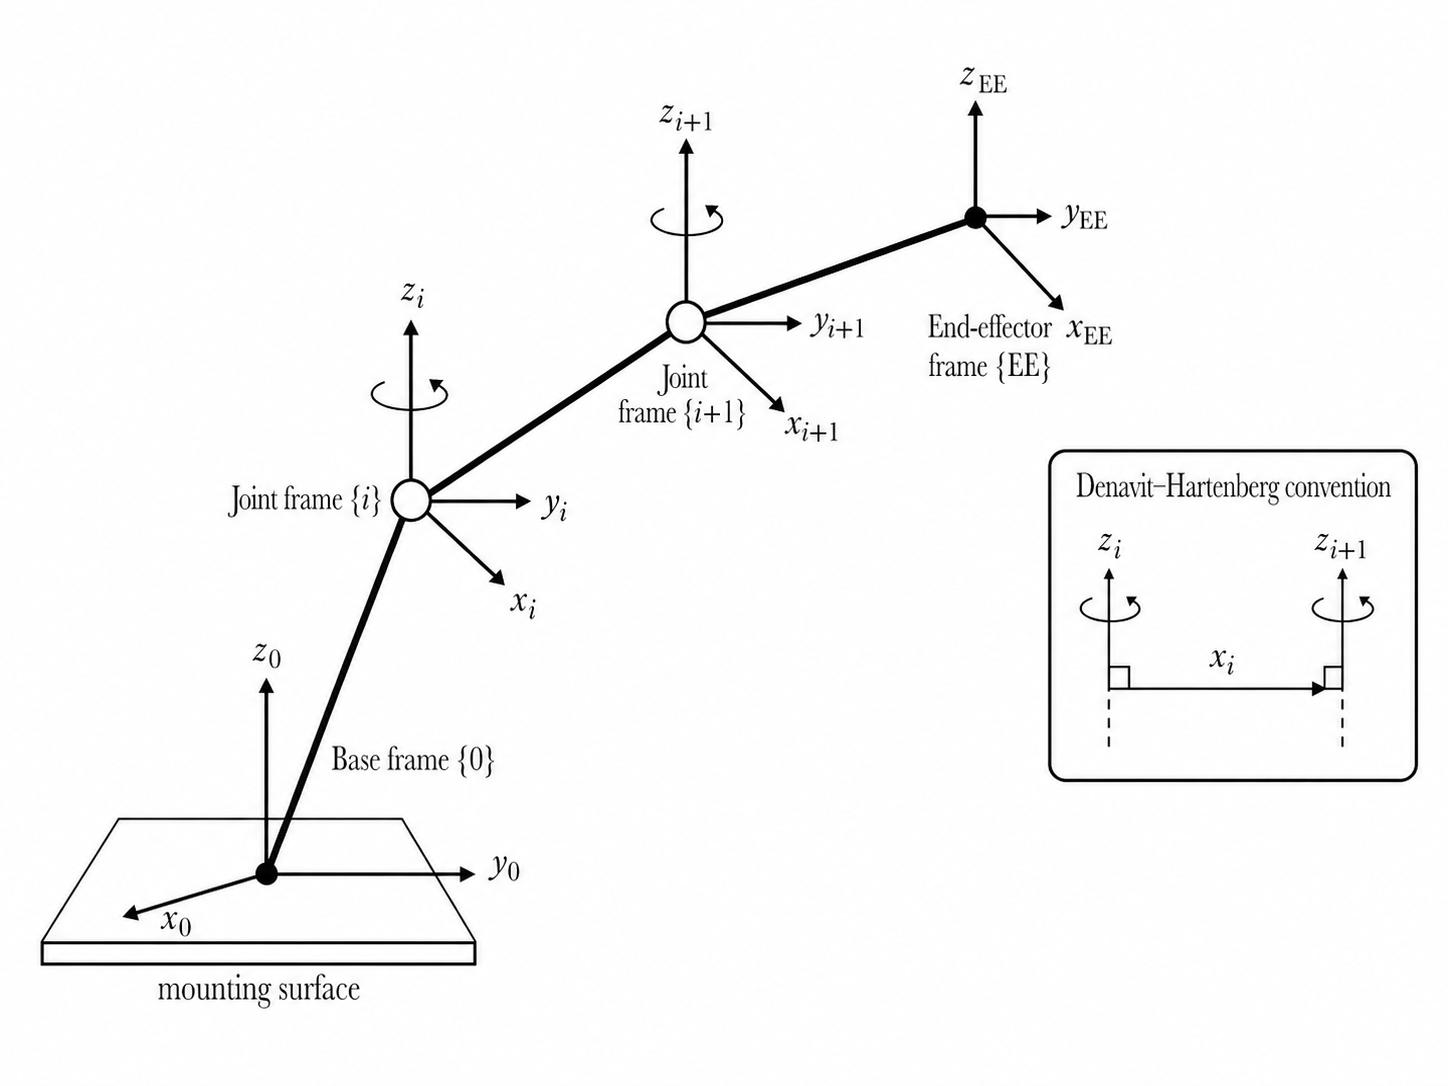
\includegraphics[width=0.95\textwidth]{figures/coordinate_frames.png}
    \caption{Coordinate-frame assignment on the left and Denavit--Hartenberg convention on the right.}
    \label{fig:coordinate_frame_robot}
\end{figure}
This frame assignment forms the basis for describing the robot kinematics using homogeneous transformation matrices.
%% ─────────────────────────────────────────────────────────────
\section{Coordinate Transformations}
\label{sec:coord_transf}
%% ─────────────────────────────────────────────────────────────

The relationship between any two coordinate frames is described by a
combination of \textbf{translation} and \textbf{rotation}
\cite{Denavit1955, Craig2005}.

\subsection{Translation}

A pure translation moves the origin of one frame to a new location
without changing its orientation.
It is represented by a position vector:

\begin{equation}
\label{eq:trans}
\mathbf{p} =
\begin{bmatrix} x \\ y \\ z \end{bmatrix}
\in \mathbb{R}^3
\end{equation}

where $x,y,z\in\mathbb{R}$ are the scalar displacements along the
three coordinate axes, measured in metres.

\subsection{Rotation Matrices}
\label{subsec:rotation}

A rotation matrix describes the orientation of one coordinate frame relative to another while leaving the origin unchanged. It therefore represents a pure change in orientation, without translation, scaling, or deformation. In three-dimensional space, rotations are commonly expressed by three successive elementary rotations about the coordinate axes.

The elementary rotations about the \(x\)-, \(y\)-, and \(z\)-axes are given by~\cite{Siciliano2009,Craig2005}:

\begin{equation}
R_x(\alpha)=
\begin{bmatrix}
1 & 0 & 0\\
0 & \cos\alpha & -\sin\alpha\\
0 & \sin\alpha & \cos\alpha
\end{bmatrix},
\label{eq:Rx}
\end{equation}

\begin{equation}
R_y(\beta)=
\begin{bmatrix}
\cos\beta & 0 & \sin\beta\\
0 & 1 & 0\\
-\sin\beta & 0 & \cos\beta
\end{bmatrix},
\label{eq:Ry}
\end{equation}

\begin{equation}
R_z(\gamma)=
\begin{bmatrix}
\cos\gamma & -\sin\gamma & 0\\
\sin\gamma & \cos\gamma & 0\\
0 & 0 & 1
\end{bmatrix}.
\label{eq:Rz}
\end{equation}

Here, \(\alpha\), \(\beta\), and \(\gamma\) denote rotations about the \(x\)-, \(y\)-, and \(z\)-axes, respectively. These angles are commonly referred to as roll, pitch, and yaw. In each elementary rotation matrix, the axis of rotation remains unchanged, while the two perpendicular axes are rotated within their plane.

In this work, the ZYX convention is used. This corresponds to applying a roll rotation about the \(x\)-axis, followed by a pitch rotation about the \(y\)-axis, and finally a yaw rotation about the \(z\)-axis~\cite{Siciliano2009,Craig2005}. The resulting rotation matrix is therefore

\begin{equation}
R = R_z(\gamma)R_y(\beta)R_x(\alpha).
\label{eq:ZYX_rotation}
\end{equation}

Expanding this product yields

\begin{equation}
R =
\begin{bmatrix}
\cos\gamma\cos\beta &
\cos\gamma\sin\beta\sin\alpha - \sin\gamma\cos\alpha &
\cos\gamma\sin\beta\cos\alpha + \sin\gamma\sin\alpha \\

\sin\gamma\cos\beta &
\sin\gamma\sin\beta\sin\alpha + \cos\gamma\cos\alpha &
\sin\gamma\sin\beta\cos\alpha - \cos\gamma\sin\alpha \\

-\sin\beta &
\cos\beta\sin\alpha &
\cos\beta\cos\alpha
\end{bmatrix}.
\label{eq:expanded_ZYX_rotation}
\end{equation}

Each element of \(R\) can be interpreted as a direction cosine. The entry \(R_{ij}\) gives the cosine of the angle between the \(i\)-th axis of the rotated frame and the \(j\)-th axis of the reference frame~\cite{Craig2005}. This interpretation is useful because it shows that the columns of \(R\) represent the rotated coordinate axes expressed in the reference frame.

A valid rotation matrix must preserve lengths and angles. This requirement leads to the orthogonality condition

\begin{equation}
R^\top R = I.
\label{eq:orthogonality_condition}
\end{equation}

As a consequence, the inverse of a rotation matrix is equal to its transpose~\cite{Siciliano2009,Murray1994},

\begin{equation}
R^{-1}=R^\top.
\label{eq:rotation_inverse}
\end{equation}

In addition, a proper rotation must have a determinant equal to one,

\begin{equation}
\det(R)=+1.
\label{eq:rotation_determinant}
\end{equation}

The determinant condition excludes reflections, which also preserve lengths and angles but reverse the handedness of the coordinate system. Together, these conditions ensure that \(R\) represents a pure rotation only.
\\
%% ─────────────────────────────────────────────────────────────
\section{Homogeneous Transformation Matrices}
\label{sec:homogeneous}
%% ─────────────────────────────────────────────────────────────
The previous sections introduced the rotation matrix for describing orientation and the translation vector for describing position. For coordinate transformations and kinematic calculations, it is often convenient to combine rotation and translation into a single representation: the homogeneous transformation matrix. This representation is particularly useful because it allows coordinate transformations and chains of frame changes to be expressed as matrix products.
This representation is widely used in robotics and kinematics because it allows consecutive coordinate transformations to be expressed as simple matrix products~\cite{Craig2005,Siciliano2009}.

The homogeneous transformation from frame \(\{a\}\) to frame \(\{b\}\) is written as

\begin{equation}
{}^bT_a =
\begin{bmatrix}
{}^bR_a & {}^bp_a\\
0^\top & 1
\end{bmatrix}
\in \mathbb{R}^{4 \times 4}.
\label{eq:homogeneous_transformation}
\end{equation}

Here, \({}^bR_a\) is the rotation matrix that describes the orientation of frame \(\{a\}\) with respect to frame \(\{b\}\).
The vector \({}^bp_a\) describes the position of the origin of frame \(\{a\}\), expressed in frame \(\{b\}\).
The last row, \(0^\top = [0 \; 0 \; 0]\) and \(1\), is introduced by the homogeneous-coordinate representation and allows rotation and translation to be combined in one matrix equation.

A point expressed in frame \(\{a\}\) can be written in homogeneous coordinates as

\begin{equation}
{}^a\tilde{p}
=
\begin{bmatrix}
{}^ap \\
1
\end{bmatrix}.
\label{eq:homogeneous_point_a}
\end{equation}

The coordinates of the same point expressed in frame \(\{b\}\) are then obtained by

\begin{equation}
{}^b\tilde{p}
=
{}^bT_a \, {}^a\tilde{p}
=
\begin{bmatrix}
{}^bR_a & {}^bp_a\\
0^\top & 1
\end{bmatrix}
\begin{bmatrix}
{}^ap\\
1
\end{bmatrix}
=
\begin{bmatrix}
{}^bR_a \, {}^ap + {}^bp_a\\
1
\end{bmatrix}.
\label{eq:homogeneous_point_transform_expanded}
\end{equation}

In non-homogeneous form, this corresponds to

\begin{equation}
{}^bp
=
{}^bR_a \, {}^ap
+
{}^bp_a.
\label{eq:non_homogeneous_transform}
\end{equation}

This equation shows that the point coordinates are first rotated into the target frame and then shifted by the translation vector between the two frame origins.

One advantage of homogeneous transformations is that several frame transformations can be composed by matrix multiplication.
For example, if a transformation from frame \(\{a\}\) to frame \(\{b\}\) is followed by a transformation from frame \(\{b\}\) to frame \(\{c\}\), the combined transformation from frame \(\{a\}\) to frame \(\{c\}\) is

\begin{equation}
{}^cT_a
=
{}^cT_b \, {}^bT_a.
\label{eq:homogeneous_composition}
\end{equation}

This property is particularly useful for kinematic chains, where the position and orientation of one frame are often obtained through a sequence of intermediate frames.

For a homogeneous transformation to describe a valid rigid-body motion, the rotation part must satisfy

\begin{equation}
R^\top R = I,
\qquad
\det(R)=1.
\label{eq:valid_rotation_conditions}
\end{equation}

These conditions ensure that the transformation preserves lengths, angles, and the handedness of the coordinate system.
Therefore, the transformation can change the position and orientation of a frame, but it cannot introduce scaling, shearing, or reflection.

The inverse transformation can also be computed efficiently.
For

\begin{equation}
T =
\begin{bmatrix}
R & p\\
0^\top & 1
\end{bmatrix},
\label{eq:general_homogeneous_transformation}
\end{equation}

the inverse is given by~\cite{Murray1994}

\begin{equation}
T^{-1}
=
\begin{bmatrix}
R^\top & -R^\top p\\
0^\top & 1
\end{bmatrix}.
\label{eq:homogeneous_inverse}
\end{equation}

This follows from the orthogonality of the rotation matrix, since \(R^{-1}=R^\top\).
As a result, inverting a homogeneous transformation requires only a transpose of the rotation matrix and one matrix-vector multiplication, rather than a general \(4 \times 4\) matrix inversion.

%% ─────────────────────────────────────────────────────────────
\section{The Controlled Variable: End-Effector Position and Orientation}
\label{sec:position_orientation}
%% ─────────────────────────────────────────────────────────────

The task of the controller is to move the end-effector to a desired position and orientation.
The position of the end-effector is described by the vector

\begin{equation}
p_{\mathrm{EE}}
=
\begin{bmatrix}
p_{x,\mathrm{EE}}\\
p_{y,\mathrm{EE}}\\
p_{z,\mathrm{EE}}
\end{bmatrix}
\in \mathbb{R}^3,
\label{eq:end_effector_position}
\end{equation}

where \(p_{x,\mathrm{EE}}\), \(p_{y,\mathrm{EE}}\), and
\(p_{z,\mathrm{EE}}\) denote the Cartesian position components of the
end-effector in the base frame.

The orientation of the end-effector is described by the rotation matrix

\begin{equation}
R_{\mathrm{EE}} \in \mathbb{R}^{3 \times 3}.
\label{eq:end_effector_rotation}
\end{equation}

Together, position and orientation describe the complete configuration of the end-effector relative to the robot base.
Since both quantities are contained in the homogeneous transformation matrix, the end-effector transformation can be written as

\begin{equation}
T_{\mathrm{EE}}
=
\begin{bmatrix}
R_{\mathrm{EE}} & p_{\mathrm{EE}}\\
0^\top & 1
\end{bmatrix}.
\label{eq:end_effector_transformation}
\end{equation}

Here, \(R_{\mathrm{EE}}\) represents the orientation of the end-effector frame with respect to the base frame, and \(p_{\mathrm{EE}}\) represents the position of the end-effector origin expressed in the base frame.
In the Franka control interface, this transformation is provided directly by \texttt{state.O\_T\_EE}.
The upper-left \(3 \times 3\) block contains the rotation matrix, while the upper-right \(3 \times 1\) block contains the Cartesian position in metres.

Using the homogeneous transformation matrix as the controlled variable is convenient because it combines position and orientation in a single representation.
It also avoids the need to describe orientation by Euler angles, which can suffer from singularities such as gimbal lock.
Since the rotation matrix is already provided directly by libfranka, no additional conversion is required.

\subsection{Position and Orientation Error}
\label{subsec:position_orientation_error}

In order to control the motion of the end-effector, the deviation between the desired and the current end-effector transformation must be computed.
Let the desired transformation be

\begin{equation}
T_d
=
\begin{bmatrix}
R_d & p_d\\
0^\top & 1
\end{bmatrix},
\label{eq:desired_transformation}
\end{equation}

and let the current end-effector transformation be

\begin{equation}
T_{\mathrm{EE}}
=
\begin{bmatrix}
R_{\mathrm{EE}} & p_{\mathrm{EE}}\\
0^\top & 1
\end{bmatrix}.
\label{eq:current_end_effector_transformation}
\end{equation}

For scalar or vector quantities, an error is usually computed by subtraction.
However, this is not suitable for homogeneous transformation matrices.
Subtracting two transformation matrices does not generally produce another meaningful rigid-body transformation.
Therefore, the error is computed using the relative transformation between the desired and the current end-effector frame.

The relative transformation is defined as

\begin{equation}
T_{\mathrm{err}}
=
T_d^{-1}T_{\mathrm{EE}}.
\label{eq:relative_transformation_error}
\end{equation}

This transformation describes the current end-effector frame relative to the desired frame.
If the current and desired end-effector transformations are identical, then

\begin{equation}
T_{\mathrm{err}}
=
T_d^{-1}T_d
=
I_4.
\label{eq:zero_transformation_error}
\end{equation}

Thus, the identity matrix represents zero position and orientation error.

Using the inverse of a homogeneous transformation, the desired inverse is

\begin{equation}
T_d^{-1}
=
\begin{bmatrix}
R_d^\top & -R_d^\top p_d\\
0^\top & 1
\end{bmatrix}.
\label{eq:desired_transformation_inverse}
\end{equation}

Substituting \(T_d^{-1}\) and \(T_{\mathrm{EE}}\) gives

\begin{equation}
T_{\mathrm{err}}
=
\begin{bmatrix}
R_d^\top & -R_d^\top p_d\\
0^\top & 1
\end{bmatrix}
\begin{bmatrix}
R_{\mathrm{EE}} & p_{\mathrm{EE}}\\
0^\top & 1
\end{bmatrix}.
\label{eq:transformation_error_product}
\end{equation}

Carrying out the block matrix multiplication yields

\begin{equation}
T_{\mathrm{err}}
=
\begin{bmatrix}
R_d^\top R_{\mathrm{EE}} & R_d^\top(p_{\mathrm{EE}}-p_d)\\
0^\top & 1
\end{bmatrix}.
\label{eq:expanded_transformation_error}
\end{equation}

The translational part of this matrix gives the position error

\begin{equation}
e_p
=
R_d^\top(p_{\mathrm{EE}}-p_d)
\in \mathbb{R}^3.
\label{eq:position_error}
\end{equation}

This error is expressed in the desired frame.
Therefore, its components describe the displacement of the current end-effector position relative to the desired frame axes.

The rotational part of the relative transformation is

\begin{equation}
\Delta R
=
R_d^\top R_{\mathrm{EE}}.
\label{eq:relative_rotation_error}
\end{equation}

This matrix describes the orientation difference between the desired and current end-effector frames.
If the current orientation is equal to the desired orientation, then \(R_{\mathrm{EE}} = R_d\), and therefore

\begin{equation}
\Delta R
=
R_d^\top R_d
=
I.
\label{eq:zero_rotation_error}
\end{equation}

Hence, the identity matrix represents zero orientation error.

For use in the impedance controller, the orientation error must be represented as a three-dimensional vector.
This is done using the axis-angle representation.
A rotation matrix \(\Delta R\) can be described by a rotation angle \(\phi\) about a rotation axis vector \(u \in \mathbb{R}^3\).
The vector \(u\) is chosen to have unit length, so it describes only the direction of the rotation axis.

The rotation angle \(\phi\) can be obtained from the trace of the relative rotation matrix \(\Delta R\).
The trace of a matrix is the sum of its diagonal elements,

\begin{equation}
\operatorname{tr}(\Delta R)
=
\Delta R_{11}
+
\Delta R_{22}
+
\Delta R_{33}.
\label{eq:rotation_trace}
\end{equation}

For a three-dimensional rotation matrix, the trace is related to the rotation angle by

\begin{equation}
\operatorname{tr}(\Delta R)
=
1 + 2\cos\phi.
\label{eq:trace_angle_relation}
\end{equation}

Solving this equation for \(\phi\) gives

\begin{equation}
\cos\phi
=
\frac{\operatorname{tr}(\Delta R)-1}{2},
\label{eq:cos_angle_from_trace}
\end{equation}

and therefore

\begin{equation}
\phi
=
\arccos
\left(
\frac{\operatorname{tr}(\Delta R)-1}{2}
\right).
\label{eq:angle_from_trace}
\end{equation}

Thus, the rotation angle can be computed directly from the diagonal elements of \(\Delta R\).

The rotation axis vector \(u\) can be obtained from the skew-symmetric part of \(\Delta R\).
This relation follows from Rodrigues' rotation formula, which expresses a rotation matrix as

\begin{equation}
\Delta R
=
I
+
\sin\phi [u]_\times
+
(1-\cos\phi)[u]_\times^2.
\label{eq:rodrigues_formula}
\end{equation}

Here, \([u]_\times\) is the skew-symmetric matrix corresponding to the rotation axis vector

\begin{equation}
u =
\begin{bmatrix}
u_x\\
u_y\\
u_z
\end{bmatrix},
\label{eq:rotation_axis_vector}
\end{equation}

and is defined as

\begin{equation}
[u]_\times
=
\begin{bmatrix}
0 & -u_z & u_y\\
u_z & 0 & -u_x\\
-u_y & u_x & 0
\end{bmatrix}.
\label{eq:skew_symmetric_axis_matrix}
\end{equation}

The term \(\sin\phi [u]_\times\) is the part of Rodrigues' formula that contains the rotation-axis information.
The factor \(\sin\phi\) appears because this skew-symmetric part of the rotation matrix depends on the sine of the rotation angle.

To isolate this part, the transpose of \(\Delta R\) is subtracted from \(\Delta R\).
Since

\begin{equation}
[u]_\times^\top = -[u]_\times,
\label{eq:skew_symmetric_property}
\end{equation}

the transpose of Rodrigues' formula is

\begin{equation}
\Delta R^\top
=
I
-
\sin\phi [u]_\times
+
(1-\cos\phi)[u]_\times^2.
\label{eq:rodrigues_transpose}
\end{equation}

Subtracting \(\Delta R^\top\) from \(\Delta R\) gives

\begin{equation}
\Delta R - \Delta R^\top
=
2\sin\phi [u]_\times.
\label{eq:skew_part_derivation}
\end{equation}

The identity terms and the symmetric term \((1-\cos\phi)[u]_\times^2\) cancel out.
Dividing by two gives the skew-symmetric part of \(\Delta R\):

\begin{equation}
\frac{1}{2}
\left(
\Delta R-\Delta R^\top
\right)
=
\sin\phi [u]_\times.
\label{eq:skew_part_rotation_matrix}
\end{equation}

This equation shows that the skew-symmetric part of \(\Delta R\) contains the rotation axis vector, scaled by \(\sin\phi\).
Therefore, to recover \(u\), the corresponding entries must be divided by \(\sin\phi\).

Reading off the entries gives

\begin{equation}
u_x =
\frac{\Delta R_{32}-\Delta R_{23}}{2\sin\phi},
\label{eq:rotation_axis_x}
\end{equation}

\begin{equation}
u_y =
\frac{\Delta R_{13}-\Delta R_{31}}{2\sin\phi},
\label{eq:rotation_axis_y}
\end{equation}

and

\begin{equation}
u_z =
\frac{\Delta R_{21}-\Delta R_{12}}{2\sin\phi}.
\label{eq:rotation_axis_z}
\end{equation}

Therefore, the rotation axis vector is

\begin{equation}
u
=
\frac{1}{2\sin\phi}
\begin{bmatrix}
\Delta R_{32}-\Delta R_{23}\\
\Delta R_{13}-\Delta R_{31}\\
\Delta R_{21}-\Delta R_{12}
\end{bmatrix}.
\label{eq:rotation_axis_from_matrix}
\end{equation}

The rotational error vector is then defined as the rotation axis vector scaled by the rotation angle:

\begin{equation}
e_R
=
\phi u.
\label{eq:rotation_error_axis_angle}
\end{equation}

Substituting the expression for \(u\) gives

\begin{equation}
e_R
=
\frac{\phi}{2\sin\phi}
\begin{bmatrix}
\Delta R_{32}-\Delta R_{23}\\
\Delta R_{13}-\Delta R_{31}\\
\Delta R_{21}-\Delta R_{12}
\end{bmatrix}
\in \mathbb{R}^3.
\label{eq:rotation_error_vector}
\end{equation}

The direction of \(e_R\) gives the axis of the required rotational correction, while its magnitude gives the orientation error in radians.
If the desired and current orientations are equal, then \(\Delta R = I\), \(\phi = 0\), and \(e_R = 0\).
For angles close to \(\pi\), the expression becomes numerically sensitive because \(\sin\phi\) approaches zero.
This case is therefore handled separately in the implementation.

Finally, the complete Cartesian error vector used by the impedance controller is obtained by stacking the translational and rotational errors:

\begin{equation}
e
=
\begin{bmatrix}
e_p\\
e_R
\end{bmatrix}
\in \mathbb{R}^6.
\label{eq:cartesian_error_vector}
\end{equation}

This vector contains the three position-error components and the three orientation-error components of the end-effector.
It therefore provides a compact representation of the deviation between the desired and current end-effector configuration.

%% ─────────────────────────────────────────────────────────────
\section{Forward Kinematics}
%% ─────────────────────────────────────────────────────────────

After defining the end-effector position and orientation as the controlled
variable, the next step is to describe how these quantities are obtained from
the robot joint angles.
This relationship is given by forward kinematics, which maps the joint
configuration of the robot to the corresponding end-effector transformation.

Forward kinematics describes the relationship between the robot joint
configuration and the resulting end-effector position and orientation.
For a serial robot manipulator, the end-effector transformation is obtained by
multiplying the homogeneous transformation matrices between neighboring link
frames.

For a robot with \(n\) joints, the forward kinematics can be written as

\begin{equation}
{}^0T_n(q)
=
{}^0T_1(q_1)
{}^1T_2(q_2)
\cdots
{}^{n-1}T_n(q_n).
\label{eq:forward_kinematics_chain}
\end{equation}

Here, \(q\) denotes the joint configuration vector,

\begin{equation}
q =
\begin{bmatrix}
q_1 & q_2 & \cdots & q_n
\end{bmatrix}^\top
\in \mathbb{R}^n.
\label{eq:joint_configuration_vector}
\end{equation}

The vector \(q\) contains the joint angles of the robot.
According to the Denavit--Hartenberg convention, each component \(q_i\)
denotes the amount of rotation of joint \(i\) about its local joint axis
\(z_i\).
The angle \(q_i\) is measured in radians.

Each matrix \({}^{i-1}T_i(q_i)\) describes the relative position and
orientation between two neighboring link frames.
In the standard Denavit--Hartenberg convention, this transformation is
obtained as a product of four elementary homogeneous transformations:

\begin{equation}
{}^{i-1}T_i(q_i)
=
R_z(q_i)\,T_z(d_i)\,T_x(a_i)\,R_x(\alpha_i).
\label{eq:dh_elementary_transformations}
\end{equation}

Here, \(R_z(q_i)\) and \(R_x(\alpha_i)\) are homogeneous rotation matrices,
while \(T_z(d_i)\) and \(T_x(a_i)\) are homogeneous translation matrices.
All four matrices have dimension \(4 \times 4\), so their product gives the
homogeneous transformation from frame \(\{i\}\) to frame \(\{i-1\}\).

Since column vectors are used, the transformations act from right to left when
applied to a point.
Thus, \(R_x(\alpha_i)\) represents the rotation about the \(x\)-axis by the
link twist angle \(\alpha_i\).
The translation \(T_x(a_i)\) then represents the displacement along the
\(x\)-axis by the link length \(a_i\).
The translation \(T_z(d_i)\) represents the displacement along the \(z\)-axis
by the offset \(d_i\).
Finally, \(R_z(q_i)\) represents the joint rotation about the local \(z\)-axis
by the joint angle \(q_i\).

Written as a single homogeneous transformation matrix, this product becomes

\begin{equation}
{}^{i-1}T_i(q_i)
=
\begin{bmatrix}
\cos q_i & -\sin q_i\cos\alpha_i & \sin q_i\sin\alpha_i & a_i\cos q_i\\
\sin q_i & \cos q_i\cos\alpha_i & -\cos q_i\sin\alpha_i & a_i\sin q_i\\
0 & \sin\alpha_i & \cos\alpha_i & d_i\\
0 & 0 & 0 & 1
\end{bmatrix}.
\label{eq:dh_transformation_matrix}
\end{equation}

The remaining Denavit–Hartenberg parameters \(d_i\), \(a_i\), and \(\alpha_i\) describe the fixed
geometry between neighboring link frames.
The parameter \(d_i\) describes a translation along the \(z\)-axis, and
\(a_i\) describes a translation along the \(x\)-axis.
The parameter \(\alpha_i\), called the link twist, describes the angle between
two neighboring joint axes.
More precisely, \(\alpha_i\) describes how much the axis \(z_i\) is tilted
with respect to the previous axis \(z_{i-1}\), as illustrated in
\cref{fig:dh_parameters}.

\begin{figure}[H]
    \centering
    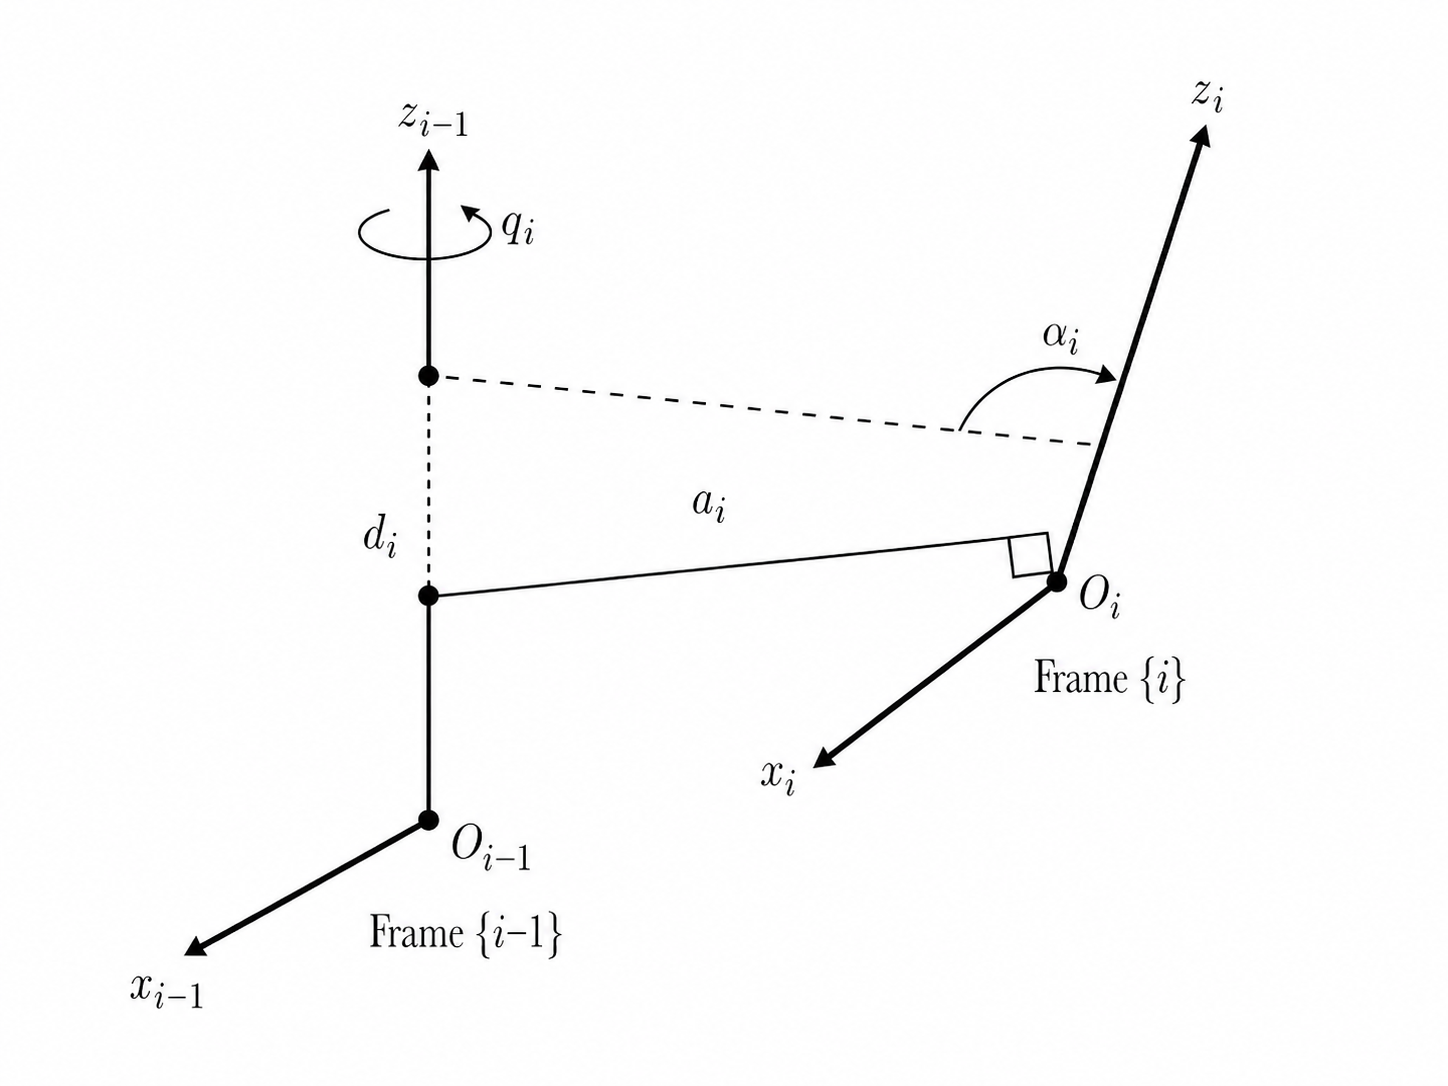
\includegraphics[width=0.75\textwidth]{figures/DH_parameters.png}
    \caption{Denavit--Hartenberg parameters between neighboring link frames.}
    \label{fig:dh_parameters}
\end{figure}

The final transformation \({}^0T_n(q)\) describes the position and orientation
of the end-effector frame with respect to the robot base frame.
It can therefore be written as

\begin{equation}
{}^0T_n(q)
=
T_{\mathrm{EE}}(q)
=
\begin{bmatrix}
R_{\mathrm{EE}}(q) & p_{\mathrm{EE}}(q)\\
0^\top & 1
\end{bmatrix}.
\label{eq:forward_kinematics_result}
\end{equation}

The upper-left \(3 \times 3\) block contains the end-effector orientation
\(R_{\mathrm{EE}}(q)\), while the upper-right \(3 \times 1\) column contains
the end-effector position \(p_{\mathrm{EE}}(q)\).

This mapping is nonlinear because the individual link transformations contain
trigonometric functions of the joint angles.
Therefore, a change in a joint angle generally produces a nonlinear change in
the end-effector position and orientation.

%% ─────────────────────────────────────────────────────────────
Forward kinematics describes how the end-effector position and orientation are
obtained from the joint angles.
For control, however, it is also necessary to describe how changes in the joint
angles affect the motion of the end-effector.
This leads to differential kinematics, which relates joint velocities to
Cartesian velocities.

\section{Differential Kinematics}
%% ─────────────────────────────────────────────────────────────

Forward kinematics provides the end-effector position and orientation as a
function of the joint configuration \(q\).
However, in control applications, the velocity relationship is also required.
Differential kinematics describes how the end-effector velocity changes with
respect to the joint velocities.

Let the Cartesian end-effector state be written as

\begin{equation}
x = f(q),
\label{eq:cartesian_state_forward_kinematics}
\end{equation}

where \(x\) represents the Cartesian position and orientation of the
end-effector, and \(q\) is the joint configuration vector.
Differentiating this relationship with respect to time gives

\begin{equation}
\dot{x}
=
J(q)\dot{q}.
\label{eq:differential_kinematics}
\end{equation}

Here, \(\dot{x} \in \mathbb{R}^6\) is the Cartesian velocity vector of the
end-effector.
It consists of the linear velocity and angular velocity,

\begin{equation}
\dot{x}
=
\begin{bmatrix}
\dot{p}_{\mathrm{EE}}\\
\omega_{\mathrm{EE}}
\end{bmatrix},
\label{eq:cartesian_velocity_vector}
\end{equation}

where \(\dot{p}_{\mathrm{EE}} \in \mathbb{R}^3\) is the linear velocity of the
end-effector and \(\omega_{\mathrm{EE}} \in \mathbb{R}^3\) is its angular
velocity.

The vector \(\dot{q} \in \mathbb{R}^n\) contains the joint velocities of the
robot,

\begin{equation}
\dot{q}
=
\begin{bmatrix}
\dot{q}_1 & \dot{q}_2 & \cdots & \dot{q}_n
\end{bmatrix}^\top,
\label{eq:joint_velocity_vector}
\end{equation}

where each \(\dot{q}_i\) describes the angular velocity of joint \(i\),
measured in radians per second.

The matrix \(J(q) \in \mathbb{R}^{6 \times n}\) is the geometric Jacobian.
It maps joint velocities to the corresponding Cartesian velocity of the
end-effector at the current configuration \(q\).
Since the Jacobian depends on \(q\), the same joint velocity can produce
different end-effector velocities depending on the current robot configuration.

%% ─────────────────────────────────────────────────────────────
The previous section introduced the velocity relation between joint space and
Cartesian space.
The matrix that describes this relation is the Jacobian.
It determines how each individual joint velocity contributes to the linear and
angular velocity of the end-effector.

\section{Jacobian Matrix}
%% ─────────────────────────────────────────────────────────────

The Jacobian matrix describes the local relationship between joint velocities
and the Cartesian velocity of the end-effector.
It appears in the differential kinematics equation

\begin{equation}
\dot{x} = J(q)\dot{q}.
\label{eq:jacobian_velocity_relation}
\end{equation}

For a robot with \(n\) joints, the geometric Jacobian is written as

\begin{equation}
J(q)
=
\begin{bmatrix}
J_1 & J_2 & \cdots & J_n
\end{bmatrix}
\in \mathbb{R}^{6 \times n}.
\label{eq:geometric_jacobian}
\end{equation}

Each column \(J_i\) describes the contribution of joint \(i\) to the
end-effector velocity.
Since the Franka Emika Panda consists of rotational joints, the \(i\)-th
column of the Jacobian is given by

\begin{equation}
J_i
=
\begin{bmatrix}
z_i \times \left(p_{\mathrm{EE}} - p_i\right)\\
z_i
\end{bmatrix}
\in \mathbb{R}^6.
\label{eq:jacobian_column}
\end{equation}

Here, \(z_i \in \mathbb{R}^3\) is the unit vector along the rotation axis of
joint \(i\), expressed in the base frame.
It is obtained from the corresponding transformation matrix as the \(z\)-axis
of frame \(\{i\}\).
The vector \(p_i \in \mathbb{R}^3\) is the position of frame \(\{i\}\),
expressed in the base frame, and \(p_{\mathrm{EE}} \in \mathbb{R}^3\) is the
end-effector position.

The vector

\begin{equation}
p_{\mathrm{EE}} - p_i
\label{eq:lever_arm}
\end{equation}

is the lever arm from joint \(i\) to the end-effector.
The cross product

\begin{equation}
z_i \times \left(p_{\mathrm{EE}} - p_i\right)
\label{eq:linear_velocity_contribution}
\end{equation}

therefore gives the linear velocity contribution at the end-effector caused by
the rotation of joint \(i\).
The lower part of the column, \(z_i\), gives the corresponding angular
velocity contribution.

Thus, each Jacobian column consists of two parts:

\begin{equation}
J_i
=
\begin{bmatrix}
\text{linear velocity contribution}\\
\text{angular velocity contribution}
\end{bmatrix}.
\label{eq:jacobian_column_parts}
\end{equation}

Because \(z_i\), \(p_i\), and \(p_{\mathrm{EE}}\) all depend on the current
joint configuration, the Jacobian is configuration-dependent.
Therefore, the influence of each joint on the end-effector motion changes as
the robot moves.

%% ─────────────────────────────────────────────────────────────
\section{Impedance Control}
%% ─────────────────────────────────────────────────────────────

The previous section introduced the Jacobian matrix, which relates joint
velocities to Cartesian end-effector velocities.
In the controller, this relationship is also used to map Cartesian forces and
moments to joint torques \cite{Khatib1987}.
Before this mapping is introduced, the desired Cartesian interaction behavior
is defined using impedance control.

Impedance control imposes a desired dynamic behavior between the end-effector
motion and the forces acting on it \cite{Hogan1985,Ott2008}.
Instead of commanding only a desired position, the robot is made to behave like
a virtual spring-damper system in Cartesian space.
In this way, deviations from the desired position and orientation generate
restoring forces and moments, while the damping terms reduce oscillations and
dissipate energy.

The Cartesian error vector was defined as

\begin{equation}
e
=
\begin{bmatrix}
e_p\\
e_R
\end{bmatrix}
\in \mathbb{R}^6,
\label{eq:cartesian_error_impedance}
\end{equation}

where \(e_p\) is the translational error and \(e_R\) is the rotational error.
These two error components are used to compute the Cartesian impedance forces
and moments.

\subsection{Impedance Forces and Moments}

The positional impedance force is defined as

\begin{equation}
f
=
K_p e_p
-
D_p \dot{p}_{\mathrm{EE}}
\in \mathbb{R}^3.
\label{eq:positional_impedance_force}
\end{equation}

Here, \(K_p \in \mathbb{R}^{3 \times 3}\) is the positional stiffness
matrix and \(D_p \in \mathbb{R}^{3 \times 3}\) is the positional damping
matrix.
The stiffness term \(K_p e_p\) generates a restoring force proportional to the
position error, while the damping term \(D_p \dot{p}_{\mathrm{EE}}\) opposes
the Cartesian linear velocity of the end-effector.

The rotational impedance moment is defined as

\begin{equation}
m
=
K_R e_R
-
D_R \omega_{\mathrm{EE}}
\in \mathbb{R}^3.
\label{eq:rotational_impedance_moment}
\end{equation}

Here, \(K_R \in \mathbb{R}^{3 \times 3}\) is the rotational stiffness matrix
and \(D_R \in \mathbb{R}^{3 \times 3}\) is the rotational damping matrix.
The stiffness term \(K_R e_R\) generates a restoring moment proportional to the
orientation error, while the damping term \(D_R \omega_{\mathrm{EE}}\) opposes
the angular velocity of the end-effector.

The positional force and rotational moment are combined into the Cartesian
force/moment vector

\begin{equation}
F
=
\begin{bmatrix}
f\\
m
\end{bmatrix}
=
\begin{bmatrix}
K_p e_p - D_p \dot{p}_{\mathrm{EE}}\\
K_R e_R - D_R \omega_{\mathrm{EE}}
\end{bmatrix}
\in \mathbb{R}^6.
\label{eq:cartesian_force_moment_vector}
\end{equation}

The vector \(F\) therefore contains the Cartesian forces and moments generated
by the impedance controller in response to position, orientation, linear
velocity, and angular velocity errors.
This force/moment vector is later mapped to joint torques using the transpose
of the Jacobian.


\subsection{Stiffness and Damping Matrices in the End-Effector Frame and Base Frame}
\label{subsec:KD_matrices}

The positional stiffness matrix \(K_p\) and damping matrix \(D_p\) do not have
to be diagonal in the robot base frame \(\{0\}\).
Here, the subscript \(p\) refers to the positional part of the impedance
controller.
A diagonal matrix is obtained only when the coordinate axes of the chosen frame
are aligned with the principal stiffness directions.
For this reason, the positional stiffness and damping matrices are first
defined in the end-effector frame \(\{\mathrm{EE}\}\), where the principal
directions are easier to specify, and are then transformed into the base frame
\(\{0\}\).

Let the orientation of the end-effector frame \(\{\mathrm{EE}\}\) with respect
to the base frame \(\{0\}\) be given by

\begin{equation}
R_{\mathrm{EE}}
=
\begin{bmatrix}
x_{\mathrm{EE}} &
y_{\mathrm{EE}} &
z_{\mathrm{EE}}
\end{bmatrix}.
\label{eq:ee_axes_in_base}
\end{equation}

The vectors \(x_{\mathrm{EE}}\), \(y_{\mathrm{EE}}\), and \(z_{\mathrm{EE}}\)
denote the unit direction vectors of the \(x\)-, \(y\)-, and \(z\)-axes of the
end-effector frame, expressed in the base frame.
They should not be confused with the Cartesian position components of the
end-effector.

In the end-effector frame, the positional stiffness matrix is chosen diagonal:

\begin{equation}
K_{p,\mathrm{EE}}
=
\operatorname{diag}(K_1,K_2,K_3)
=
\begin{bmatrix}
K_1 & 0 & 0\\
0 & K_2 & 0\\
0 & 0 & K_3
\end{bmatrix}.
\label{eq:positional_stiffness_ee}
\end{equation}

Here, \(K_1\), \(K_2\), and \(K_3\) are positive stiffness values along the
\(x\)-, \(y\)-, and \(z\)-axes of the end-effector frame, respectively.
If all three values are equal, the virtual spring has the same stiffness in
every direction.
If the values are different, the stiffness depends on direction.

Since the impedance force is computed in the base frame, the stiffness matrix
must also be expressed in the base frame.
This is done by rotating the stiffness matrix from the end-effector frame into
the base frame:

\begin{equation}
K_{p,0}
=
R_{\mathrm{EE}}
K_{p,\mathrm{EE}}
R_{\mathrm{EE}}^\top .
\label{eq:positional_stiffness_base}
\end{equation}

This equation shows that the stiffness matrix can be diagonal in the
end-effector frame but become a full matrix in the base frame.
The off-diagonal terms are not errors; they describe coupling between the
base-frame directions caused by the orientation of the end-effector frame.

Equivalently, the stiffness matrix in the base frame can be written as

\begin{equation}
K_{p,0}
=
K_1\,x_{\mathrm{EE}}x_{\mathrm{EE}}^\top
+
K_2\,y_{\mathrm{EE}}y_{\mathrm{EE}}^\top
+
K_3\,z_{\mathrm{EE}}z_{\mathrm{EE}}^\top .
\label{eq:positional_stiffness_dyadic}
\end{equation}

This form shows how each end-effector axis contributes to the full stiffness
matrix in the base frame.

The damping matrix is constructed in the same way.
In the end-effector frame, it is chosen as

\begin{equation}
D_{p,\mathrm{EE}}
=
\operatorname{diag}(D_1,D_2,D_3).
\label{eq:positional_damping_ee}
\end{equation}

For a unit virtual mass in each principal direction, critical damping gives

\begin{equation}
D_i = 2\sqrt{K_i},
\qquad i=1,2,3.
\label{eq:critical_damping}
\end{equation}

Thus,

\begin{equation}
D_{p,\mathrm{EE}}
=
2\operatorname{diag}
\left(
\sqrt{K_1},
\sqrt{K_2},
\sqrt{K_3}
\right).
\label{eq:positional_damping_ee_critical}
\end{equation}

The damping matrix expressed in the base frame is then

\begin{equation}
D_{p,0}
=
R_{\mathrm{EE}}
D_{p,\mathrm{EE}}
R_{\mathrm{EE}}^\top .
\label{eq:positional_damping_base}
\end{equation}

The same construction can be applied to the rotational stiffness matrix
\(K_{R,0}\) and the rotational damping matrix \(D_{R,0}\).
In this case, rotational stiffness is expressed in \(\mathrm{Nm/rad}\),
whereas positional stiffness is expressed in \(\mathrm{N/m}\).

%% ─────────────────────────────────────────────────────────────
\section{Control Law}
\label{sec:control_law}
%% ─────────────────────────────────────────────────────────────

After defining the Cartesian impedance forces and moments, the final step is
to convert them into joint torques that can be commanded to the robot
actuators.
This mapping is performed using the transpose of the Jacobian
\cite{Khatib1987}.

The Cartesian force/moment vector is given by

\begin{equation}
F =
\begin{bmatrix}
f\\
m
\end{bmatrix}
\in \mathbb{R}^6,
\label{eq:cartesian_force_moment_control_law}
\end{equation}

where \(f \in \mathbb{R}^3\) is the Cartesian force and
\(m \in \mathbb{R}^3\) is the Cartesian moment.
Using the principle of virtual work, this vector is mapped to joint torques
\cite{Khatib1987} by

\begin{equation}
\tau
=
J^\top(q)F.
\label{eq:joint_torque_mapping}
\end{equation}

Here, \(\tau \in \mathbb{R}^n\) is the joint torque vector,

\begin{equation}
\tau =
\begin{bmatrix}
\tau_1 & \tau_2 & \cdots & \tau_n
\end{bmatrix}^\top,
\label{eq:joint_torque_vector}
\end{equation}

where each \(\tau_i\) is measured in \(\mathrm{Nm}\).
The matrix \(J^\top(q) \in \mathbb{R}^{n \times 6}\) is the transpose of the
Jacobian and maps the Cartesian force/moment vector into joint torques.

Substituting the Cartesian impedance forces and moments gives the complete
Cartesian impedance control law:

\begin{equation}
\tau
=
J^\top(q)
\begin{bmatrix}
K_{p,0} e_p - D_{p,0} \dot{p}_{\mathrm{EE}}\\
K_{R,0} e_R - D_{R,0} \omega_{\mathrm{EE}}
\end{bmatrix}.
\label{eq:cartesian_impedance_control_law}
\end{equation}

This equation is the computational core of the controller.
At each control cycle, the current end-effector transformation is read from
the robot state and compared with the desired transformation.
From this comparison, the positional error \(e_p\) and rotational error
\(e_R\) are computed.
The corresponding Cartesian forces and moments are then evaluated and mapped
to joint torques using the Jacobian transpose.

\subsection{Gravity and Coriolis Compensation}

In practice, the impedance torques are combined with model-based compensation
terms.
These terms compensate for gravity and velocity-dependent effects in the robot
dynamics.
The commanded joint torque is therefore given by

\begin{equation}
\tau_{\mathrm{cmd}}
=
J^\top(q)F
+
\tau_g(q)
+
\tau_c(q,\dot{q}).
\label{eq:commanded_torque}
\end{equation}

Here, \(\tau_g(q) \in \mathbb{R}^n\) is the gravity compensation torque, which
depends on the joint configuration \(q\).
The term \(\tau_c(q,\dot{q}) \in \mathbb{R}^n\) compensates for Coriolis and
centrifugal effects, which depend on both the joint configuration \(q\) and
the joint velocity \(\dot{q}\).

These compensation terms are provided by the libfranka model interface and are
recomputed at every control step \cite{FrankaFCI2023}.
Adding them helps ensure that the commanded torque produces the desired
impedance behavior instead of being distorted by gravity or velocity-dependent
dynamic effects.
